\documentclass[11pt]{article}

\usepackage[margin=1in]{geometry}
\usepackage{amsmath,amssymb,amsthm,mathtools}
\usepackage{graphicx}
\usepackage{booktabs}
\usepackage{tikz}
\usepackage{enumitem}
\usepackage[colorlinks=true,linkcolor=blue!50!black,citecolor=blue!50!black,urlcolor=blue!50!black]{hyperref}

\emergencystretch=1.5em

\newtheorem{definition}{Definition}
\newtheorem{proposition}{Proposition}
\newtheorem{conjecture}{Conjecture}
\theoremstyle{remark}
\newtheorem{remark}{Remark}

\newcommand{\R}{\mathbb{R}}
\newcommand{\Z}{\mathbb{Z}}
\newcommand{\N}{\mathbb{N}}
\newcommand{\B}{\mathcal{B}}
\newcommand{\F}{\mathcal{F}}
\newcommand{\E}{\mathbb{E}}
\newcommand{\KL}{D_{\mathrm{KL}}}
\newcommand{\PSL}{\mathrm{PSL}}

\title{Genealogy and Time:\\[4pt]
\large Braids, Cylinders and Emergent Objects in Chaotic Dynamics}
% TODO: author name and affiliation
\author{\textit{[Author]}}
\date{October 2026}

\begin{document}
\maketitle

\begin{abstract}
Periodic solutions of the planar three-body problem, drawn as world-lines in space-time, form braids.
We use this observation, made concrete in an interactive instrument that renders the 26{,}646 published
periodic orbits as glowing trails and as braids, as the entry point to a more general account of how
discrete, identifiable \emph{forms} arise from continuous chaotic dynamics.
We show how the braid group $B_3$ organises the known topological classifications of three-body orbits
(the pure braid group $P_3\cong F_2\times\Z$ recovers Montgomery's free-group words, and free-fall orbits
have trivial full-period braid $\beta\beta^{-1}$), how the non-commutativity of time-ordered composition
appears both in symplectic integration and in braid words, and how sensitivity to initial conditions gives
forms a finite lifetime $\tau\approx\lambda^{-1}\ln(\delta/\varepsilon)$.
We compute the braid of all 14{,}473 distinct catalogued orbits and validate it against the published words and
syzygy sequences (2{,}043 of 2{,}044 and 236 of 236; the one difference is an error in the published table).
The census shows four things. The figure-eight realises the golden braid $(\sigma_1\sigma_2^{-1})^3$. Within each
mass ratio, braid entropy grows linearly with the scale-invariant period. Braid entropy is uncorrelated with the
orbit's Lyapunov exponent. Hierarchical orbits are exactly the reducible braids.
The symbolic $n$-cylinders of the dynamics carry a genealogical probability structure (a filtration,
conditional measures that are exact mixtures of their descendants, a martingale of refining predictions and
a scale decomposition of Kullback--Leibler divergence), and the tree is \emph{grown} by time rather than
given in advance: dynamical evolution acts as a refinement operator whose information production rate is the
Kolmogorov--Sinai entropy. Finally, following Poincar\'e's definition of displacement as compensable change,
we argue that what counts as a solid object depends on resolution, and that chaos makes resolution and time
dual: two parts separated by $\delta_0$ remain one object at scale $\varepsilon$ for a time
$\lambda^{-1}\ln(\varepsilon/\delta_0)$. KAM tori are the dynamical archetype of permanent objects; chaotic
layers are where objects are born and die. We separate established results from conjectures throughout and
close with a concrete computational programme.
\end{abstract}

\tableofcontents

%=====================================================================
\section{Introduction}
%=====================================================================

The three-body problem is where modern dynamics began. Poincar\'e's prize memoir on it introduced homoclinic
tangles, qualitative methods and the realisation that deterministic motion can be practically unpredictable;
the attempt to tame its perturbation series led, through Kolmogorov, Arnold and Moser, to KAM theory. It
would be a mistake to read the present paper as a statement about gravitation. The three-body problem is our
\emph{instrument}: a system rich enough to exhibit every phenomenon we discuss and documented well enough
(Section~\ref{sec:instrument}) to be checked numerically.

The thread of the paper is a single question: \emph{what is a thing, if everything is a trajectory?} We
approach it in steps.
\begin{enumerate}[leftmargin=*]
\item Trajectories of three bodies, viewed in space-time, are braids; braids are algebraic objects with
      invariants (Section~\ref{sec:braids}). We compute them for all 14{,}473 catalogued orbits
      (Section~\ref{sec:census}).
\item A braid word is a time-ordered product, and the order of composition matters, in the algebra of braids
      as in the numerical integration of Hamilton's equations (Section~\ref{sec:order}).
\item Because the dynamics is chaotic, a braid is realised only temporarily: forms are born, persist and die
      (Section~\ref{sec:forms}).
\item The symbolic cylinders that index these forms carry a genealogical probability structure
      (Section~\ref{sec:genealogy}).
\item That genealogy is not a pre-existing tree but is grown by time (Section~\ref{sec:time}).
\item What counts as an object at all depends on the scale of observation, and chaos makes scale and time
      dual (Section~\ref{sec:objects}).
\end{enumerate}
Section~\ref{sec:programme} lists the computations that would test the claims.

\paragraph{Status of claims.} We label statements as \emph{theorems} (established mathematics, with
references), \emph{numerical observations} (results obtained with the instrument), or \emph{conjectures and
proposals}. Philosophical interpretations are stated as such.

%=====================================================================
\section{The instrument: periodic three-body orbits as trails and braids}
\label{sec:instrument}
%=====================================================================

We built an interactive, browser-based gallery\footnote{Source code: \url{https://github.com/roholazandie/n-body}.}
of planar periodic solutions of Newton's equations with $G=1$,
\begin{equation}
  m_i\ddot{\mathbf r}_i=\sum_{j\neq i}\frac{m_im_j(\mathbf r_j-\mathbf r_i)}{|\mathbf r_j-\mathbf r_i|^3},
  \qquad i=1,2,3 .
\end{equation}
It plays three published catalogues.
\begin{itemize}[leftmargin=*]
\item \textbf{Classic orbits} (20): the figure-eight \cite{Moore1993,ChencinerMontgomery2000}, Lagrange's
      equilateral solution, the \v{S}uvakov--Dmitra\v{s}inovi\'c families \cite{SuvakovDmitrasinovic2013} and
      Broucke orbits.
\item \textbf{Li \& Liao} (2{,}044): 695 equal-mass and 1{,}349 unequal-mass zero-angular-momentum orbits
      from isosceles collinear initial conditions \cite{LiLiao2017,LiJingLiao2018}.
\item \textbf{Free fall} (24{,}582 initial conditions, 12{,}409 distinct solutions, 236 self-dual): equal
      masses released from rest, body 1 at a point $P(x,y)$ of the Agekyan--Anosova domain
      $D=\{x\ge0,\,y\ge0,\,(x+\tfrac12)^2+y^2\le1\}$, bodies 2 and 3 at $(\mp\tfrac12,0)$
      \cite{AgekyanAnosova1968,Hristov2024}.
\end{itemize}

\paragraph{Integration.} The orbits are violently unstable: the free-fall catalogue reports Lyapunov
multipliers up to $e^{31}$ per period \cite{Hristov2024}, and individual orbits pass within $10^{-8}$ of a
binary collision. We integrate with algorithmic regularisation \cite{MikkolaTanikawa1999a,MikkolaTanikawa1999b}:
a logarithmic-Hamiltonian leapfrog, exact for Kepler motion, in \emph{chain coordinates} (relative vectors
along the two shortest edges, so that a close pair keeps full double precision), driven by Gragg--Bulirsch--Stoer
extrapolation with exact landing on prescribed times. Free-fall orbits come to rest again at $T/2$ and then
retrace their path; we integrate $[0,T/2]$ only and mirror it.

\paragraph{Numerical observations.} (i) Every catalogued free-fall i.c.\ sampled (492 of them) reaches
$T/2$ with residual speed below $6\times10^{-4}$ (median $\sim10^{-7}$), and the scale-invariant period
$T^*=T|E|^{3/2}$ computed from the energy reproduces the catalogue. (ii) All 2{,}044 Li--Liao orbits return
to their initial state after the published period to within $6\times10^{-5}$ in phase space. (iii) Energy is
conserved to $10^{-10}$ through the closest encounter in the catalogue. (iv) Perturbing a free-fall orbit
with Lyapunov exponent $\lambda\approx15$ per period by $10^{-6}$ destroys it within one to two periods.

\paragraph{Braid view.} Besides glowing trails (Fig.~\ref{fig:instrument}, left), each orbit can be shown as
world-lines (Fig.~\ref{fig:instrument}, right): the horizontal coordinate is the position projected on an
axis at angle $\theta$, the vertical coordinate is time, and the in-plane coordinate perpendicular to the axis
is used as depth, so that at every crossing the nearer strand passes over the farther one. The time window is
measured in scale-invariant time $t^*=t|E|^{3/2}$ so that all orbits scroll at a common rate; a zoom control
compresses time linearly while narrowing the braid by the square root of the zoom factor.

\begin{figure}[t]
  \centering
  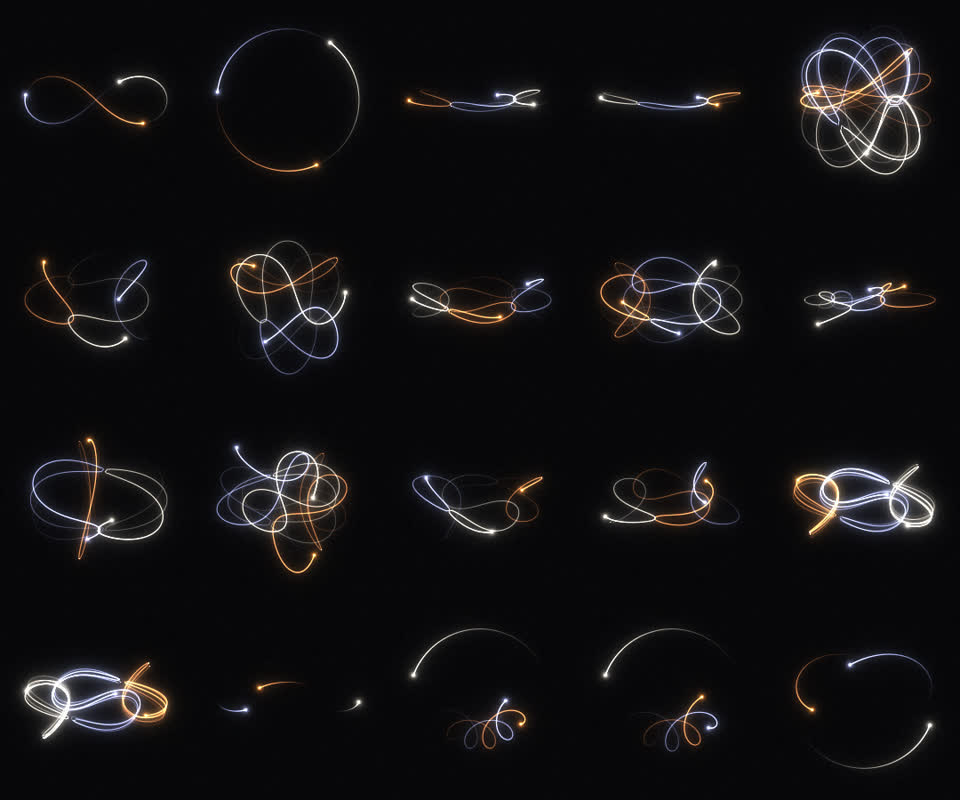
\includegraphics[width=0.49\linewidth]{docs/orbits.jpg}\hfill
  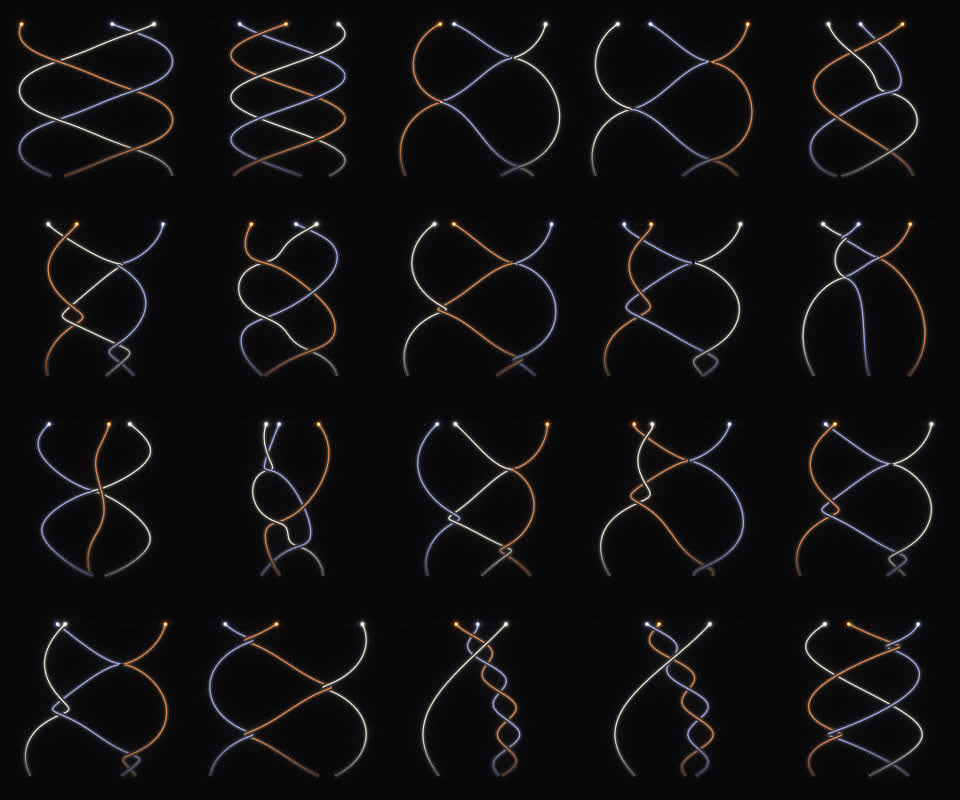
\includegraphics[width=0.49\linewidth]{docs/braids.jpg}
  \caption{The instrument. Left: twenty classic periodic orbits as trails. Right: the same orbits as braids,
  with position along a projection axis horizontally and time running upward; at each crossing the strand
  nearer the viewer passes over.}
  \label{fig:instrument}
\end{figure}

%=====================================================================
\section{Braids of three-body orbits}
\label{sec:braids}
%=====================================================================

\subsection{The braid group $B_3$ and reading a word}

The world-lines $t\mapsto(\mathbf r_i(t),t)\in\R^2\times[0,T]$ of three bodies that never collide form a
geometric braid. Its isotopy class is an element of Artin's braid group
\begin{equation}
  B_3=\langle\sigma_1,\sigma_2\mid\sigma_1\sigma_2\sigma_1=\sigma_2\sigma_1\sigma_2\rangle .
\end{equation}
To read a word, project onto a generic axis and scan upward in time. Whenever the bodies in positions $i$ and
$i+1$ of the left-to-right order exchange places, record $\sigma_i^{\varepsilon}$, with $\varepsilon=+1$ if
the strand moving rightward passes in front and $\varepsilon=-1$ otherwise. The braid is the time-ordered
product
\begin{equation}
  \beta=\sigma_{i_1}^{\varepsilon_1}\sigma_{i_2}^{\varepsilon_2}\cdots\sigma_{i_n}^{\varepsilon_n}.
  \label{eq:word}
\end{equation}

\begin{figure}[h]
\centering
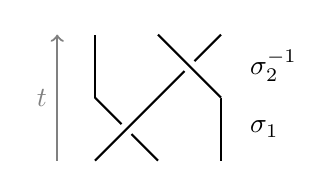
\begin{tikzpicture}[scale=0.8,thick]
  % sigma_1 : strands at x=0,1 cross, strand 2 vertical
  \draw (2,0) -- (2,1);
  \draw (1,0) -- (0,1);
  \draw[white,line width=5pt] (0,0) -- (1,1);
  \draw (0,0) -- (1,1);
  % sigma_2^{-1}
  \draw (0,1) -- (0,2);
  \draw (1,1) -- (2,2);
  \draw[white,line width=5pt] (2,1) -- (1,2);
  \draw (2,1) -- (1,2);
  \node[right] at (2.3,0.5) {$\sigma_1$};
  \node[right] at (2.3,1.5) {$\sigma_2^{-1}$};
  \draw[->,gray] (-0.6,0) -- (-0.6,2) node[midway,left] {$t$};
\end{tikzpicture}
\caption{The braid $\sigma_1\sigma_2^{-1}$, read bottom to top.}
\label{fig:golden}
\end{figure}

\begin{proposition}[Projection independence]
For a periodic orbit the world-lines close up in $\R^2\times S^1$, and the words obtained from different
generic projection angles are conjugate in $B_3$ (after the relabelling induced by the change of starting
order). The conjugacy class is therefore an invariant of the orbit.
\end{proposition}
\noindent Rotating the projection (an option in the instrument) produces many words for one invariant object.
The census of Section~\ref{sec:census} checks this numerically. At three projection angles, every one of the
14{,}473 orbits gives the same invariants.

\subsection{Relation to the established topological classifications}

Let $C_3(\R^2)$ be the space of ordered triples of distinct points in the plane. Its fundamental group is the
pure braid group $P_3=\ker(B_3\to S_3)$, and
\begin{equation}
  P_3\;\cong\;F_2\times\Z ,
  \label{eq:P3}
\end{equation}
where the central factor $\Z$ is generated by the full twist $\Delta^2=(\sigma_1\sigma_2)^3$, a rigid rotation
of the whole configuration by $2\pi$ \cite{KasselTuraev2008,Birman1974}. Quotienting $C_3(\R^2)$ by
translations, dilations and rotations leaves the shape sphere minus the three binary-collision points, whose
fundamental group is the free group $F_2$. This is the setting of Montgomery's topological classification of
three-body orbits by free-group words \cite{Montgomery1998}, used by \v{S}uvakov and Dmitra\v{s}inovi\'c and by
Li and Liao (e.g.\ $BabA$ for the figure-eight family). By \eqref{eq:P3}, \emph{those words are the
orbit's braid with the overall rotation divided out.} Moore's discovery of the figure-eight came precisely from
prescribing a braid type and searching for a gravitational orbit realising it \cite{Moore1993}.

\begin{proposition}[Free-fall braids are trivial over a full period]
\label{prop:freefall}
Free-fall orbits satisfy $\mathbf r_i(T/2+s)=\mathbf r_i(T/2-s)$. A geometric braid traversed backward in time
represents the inverse element, so the full-period braid is $\beta\,\beta^{-1}=1$.
\end{proposition}
\noindent This explains, in braid language, why Hristov et al.\ assign symbolic sequences only to the half
period and observe that the full-period sequence is trivial \cite{Hristov2024}; the invariant object is the
half-period braid between the two moments of rest.

\subsection{Invariants}

Because $B_3$ is small, its invariants are computable for every catalogued orbit.

\begin{table}[h]
\centering
\begin{tabular}{@{}ll@{}}
\toprule
Invariant & Meaning\\
\midrule
Permutation $\beta\mapsto S_3$ & whether bodies return to their own places\\
Exponent sum $\sum\varepsilon_k$ & homomorphism $B_3\to\Z$; net winding ($\Delta^2\mapsto6$)\\
Image in $\PSL(2,\Z)\cong B_3/\langle\Delta^2\rangle$ & $\sigma_1\mapsto\bigl(\begin{smallmatrix}1&1\\0&1\end{smallmatrix}\bigr)$,
  $\sigma_2\mapsto\bigl(\begin{smallmatrix}1&0\\-1&1\end{smallmatrix}\bigr)$\\
Nielsen--Thurston type & $|\mathrm{tr}|<2$ periodic, $=2$ reducible, $>2$ pseudo-Anosov\\
Dilatation $\lambda_\beta$ & largest eigenvalue; $\log\lambda_\beta$ bounds topological entropy\\
\bottomrule
\end{tabular}
\caption{Braid invariants of an orbit.}
\label{tab:invariants}
\end{table}

\noindent For example $\sigma_1\sigma_2^{-1}\mapsto\bigl(\begin{smallmatrix}2&1\\1&1\end{smallmatrix}\bigr)$,
with trace $3$ and dilatation $\varphi^2=(3+\sqrt5)/2$; this is the ``golden'' stirring braid of topological
fluid mixing \cite{BoylandArefStremler2000}. By the Nielsen--Thurston theory \cite{Thurston1988}, any
continuous motion of a surface realising a pseudo-Anosov braid has topological entropy at least
$\log\lambda_\beta$ per period: the braid forces a minimum amount of stretching on everything around it.

\noindent Whether the figure-eight is such a stirrer, and how the dilatation behaves across the catalogues, are
questions of measurement; Section~\ref{sec:census} answers them.

%=====================================================================
\section{A braid census of the catalogues}
\label{sec:census}
%=====================================================================

We computed the braid of every distinct catalogued orbit: the 20 classic orbits, the 2{,}044 Li--Liao orbits,
and one initial condition for each of the 12{,}409 distinct free-fall solutions, 14{,}473 orbits in all.
The census runs in about a minute on a laptop (\texttt{scripts/braid-census.js}), and its results can be
explored in the instrument's ``Braid lab'' view (Fig.~\ref{fig:census}).

\subsection{Method}

\paragraph{Dense trajectories.} Each orbit is integrated with the regularised scheme of
Section~\ref{sec:instrument} at tolerance $10^{-12}$, with two step limits: $\Delta t\le T/3000$, and
$\Delta t\le0.08\,r_{\min}^{3/2}/\sqrt{M}$, where $r_{\min}$ is the smallest pair distance and $M$ the total
mass, so that a close binary turns through at most a fraction of a radian per step. Within a step, positions are
interpolated by cubic Hermite polynomials.

\paragraph{Syzygies and free-group words.} Collinear configurations are the zeros of the signed area of the
triangle. Each sign change is located by sub-sampling followed by bisection, and records which body lies in the
middle and the crossing direction. Following Montgomery \cite{Montgomery1998}, the syzygy sequence is
converted into a word in $F_2=\langle a,b\rangle$ by recording crossings of the two equatorial arcs on which
body 1 or body 2 is in the middle, and the word is cyclically reduced.

\paragraph{Braid words and invariants.} The braid word \eqref{eq:word} is read from the world-lines projected
on an axis at angle $\theta$, with the in-plane normal coordinate as depth. It is freely reduced and mapped to
$\PSL(2,\Z)$ in exact integer arithmetic; traces reach 168 decimal digits. The central image $\pm I$ (for
example the full twist $\Delta^2$) is classed as periodic.

\paragraph{Closure.} A closed orbit that starts in a collinear configuration (the figure-eight, Li--Liao
orbits) would put a syzygy on the boundary of $[0,T]$. We therefore integrate over $[0,T+2\delta]$ with
$\delta=10^{-3}T$ and use the shifted window $(\delta,T+\delta]$. Free-fall orbits have trivial full-period
braid (Proposition~\ref{prop:freefall}); for them we use the half-period braid, closed by a straight-line return
from the configuration at $T/2$ to the initial one. This is a choice of closure, analogous to the great-circle
closure of Ref.~\cite{Hristov2024}, and numbers for free-fall orbits refer to it.

\subsection{Validation}

\begin{table}[h]
\centering
\begin{tabular}{@{}lr@{}}
\toprule
Check & Agreement\\
\midrule
Li--Liao free-group words, up to cyclic permutation and inversion \cite{LiLiao2017,LiJingLiao2018} & 2{,}043 / 2{,}044\\
Self-dual free-fall half-period syzygy sequences, same body labels \cite{Hristov2024} & 236 / 236\\
Same $|\mathrm{tr}|$ (hence type and $\lambda$) at projection angles $\theta=0.31,1.13,2.02$ & 14{,}473 / 14{,}473\\
Braid trace equals the trace of the $F_2$ word under $a\mapsto\sigma_1^2,\ b\mapsto\sigma_2^{-2}$ (sampled) & 82 / 82\\
\bottomrule
\end{tabular}
\caption{Validation of the census against published topology and against itself.}
\label{tab:validation}
\end{table}

The published Li--Liao tables contain three entries that differ from our computed words. Two of them (II.D 1
and II.D 2) are not freely reduced and reduce to the empty word, which is what we compute; we therefore compare
freely reduced words. The third (I.B 33, $m_3=2$) is one letter shorter than the word length $L_f$ listed in the
same table for that orbit, so we take it to be a transcription error. The last row of Table~\ref{tab:validation}
checks two independent routes against each other. The syzygy route and the projection route meet through
$P_3\cong F_2\times\Z$ \eqref{eq:P3}, and since the congruence subgroup $\Gamma(2)$ is the image of $P_3$, the
two traces must agree.

\subsection{Results}

\begin{proposition}[The figure-eight is a golden stirrer; numerical]
\label{prop:fig8}
The braid of the figure-eight orbit is $(\sigma_1\sigma_2^{-1})^3$ up to conjugation, with $|\mathrm{tr}|=18$
and $\log\lambda_\beta=3\log\varphi^2\approx2.887$. Its syzygy sequence is $123123$.
\end{proposition}
\noindent Among free-fall orbits, the half-period braid of the simplest self-dual orbit closes to the same
element, $(\sigma_2^{-1}\sigma_1)^3$.

\paragraph{Nielsen--Thurston types.} Almost every orbit is pseudo-Anosov
(Table~\ref{tab:types}). The exceptions are informative. Lagrange's rigid rotation is periodic, its braid a
power of the full twist with exponent sum $\pm6$. The four Broucke orbits are reducible: a tight binary is
orbited by the third body, so an invariant curve encloses the binary. This is exactly the ``aggregate'' of
Section~\ref{sec:forms}. Two Li--Liao orbits (II.D 1 and 2) have trivial braid despite having 14 and 22
syzygies, because their syzygy sequences cancel in $F_2$.

\begin{table}[h]
\centering
\begin{tabular}{@{}lrrrr@{}}
\toprule
 & periodic & reducible & pseudo-Anosov & total\\
\midrule
Classic & 1 & 4 & 15 & 20\\
Li--Liao & 2 & 0 & 2{,}042 & 2{,}044\\
Free fall (half period, closed) & 1 & 89 & 12{,}319 & 12{,}409\\
\bottomrule
\end{tabular}
\caption{Nielsen--Thurston types of the catalogued orbits.}
\label{tab:types}
\end{table}

\paragraph{Entropy per crossing is at most $\log\varphi$.} Across all 14{,}376 pseudo-Anosov braids,
$\log\lambda_\beta$ divided by the number of crossings of the reduced word never exceeds
$\log\varphi\approx0.4812$, and it reaches this value only for powers of the golden braid. This agrees with the
known optimality of $\sigma_1\sigma_2^{-1}$ among three-strand braids with respect to entropy per generator
\cite{DAlessandro1999,FinnThiffeault2011}. It is a consistency check, not a discovery. Measured against the
bound, the Li--Liao orbits are efficient stirrers, with median $0.38$ per crossing, $79\%$ of the maximum.

\paragraph{A topological Kepler law.} Kepler's third law ties a period to a size. Here the period ties to
topological complexity. Pooled over the whole Li--Liao catalogue, the Spearman correlation between
$\log\lambda_\beta$ and $T^*$ is only $0.85$. The pooled scatter, however, separates into distinct curves
(Fig.~\ref{fig:census}, left), one for each mass ratio $m_3$. Within each mass class the relation is linear
to high accuracy:
\begin{equation}
  \log\lambda_\beta\;\approx\;\kappa(m_3)\,T^*,\qquad \text{Pearson } r\ge0.997 \text{ for every } m_3,
  \label{eq:kepler}
\end{equation}
with $\kappa=0.313$ for equal masses and $m_3\,\kappa(m_3)$ between $0.29$ and $0.32$ for all eight mass ratios
$m_3\in\{0.5,0.75,1,2,4,5,8,10\}$. Word length is equally linear in $T^*$ within a mass class (Spearman
$\ge0.98$), so \eqref{eq:kepler} is also a statement that topological entropy grows in proportion to word length,
at an almost fixed fraction of the golden bound. We have no derivation of the approximate $1/m_3$ scaling.
Part of it may come from $T^*=T|E|^{3/2}$, which is not normalised by mass. The classic orbits follow the same
line as the equal-mass Li--Liao orbits ($\log\lambda_\beta\approx0.33\,T^*-1.6$, Spearman $0.98$). For free-fall
half-period braids, the entropy per unit of full-period $T^*$ is lower (median $0.12$) and more dispersed.

\paragraph{Braid entropy is not instability.} For the free-fall orbits we can compare $\log\lambda_\beta$ with
the Lyapunov exponent of the orbit itself, as published in Ref.~\cite{Hristov2024}. The two are essentially
uncorrelated: Spearman $\rho=-0.17$ over 12{,}409 orbits (Fig.~\ref{fig:census}, right), and the Lyapunov
exponent is also uncorrelated with $T^*$ ($\rho=0.06$). The two numbers measure different things. The Lyapunov
exponent is the instability of the orbit, the rate at which a neighbouring trajectory leaves it. The braid
entropy is a lower bound on the stretching that the orbit forces on every surrounding motion. An orbit can be
very unstable and topologically simple, or the reverse. In the language of
Section~\ref{sec:forms}, the lifetime of a form and the complexity of the form are independent coordinates.

\begin{figure}[t]
  \centering
  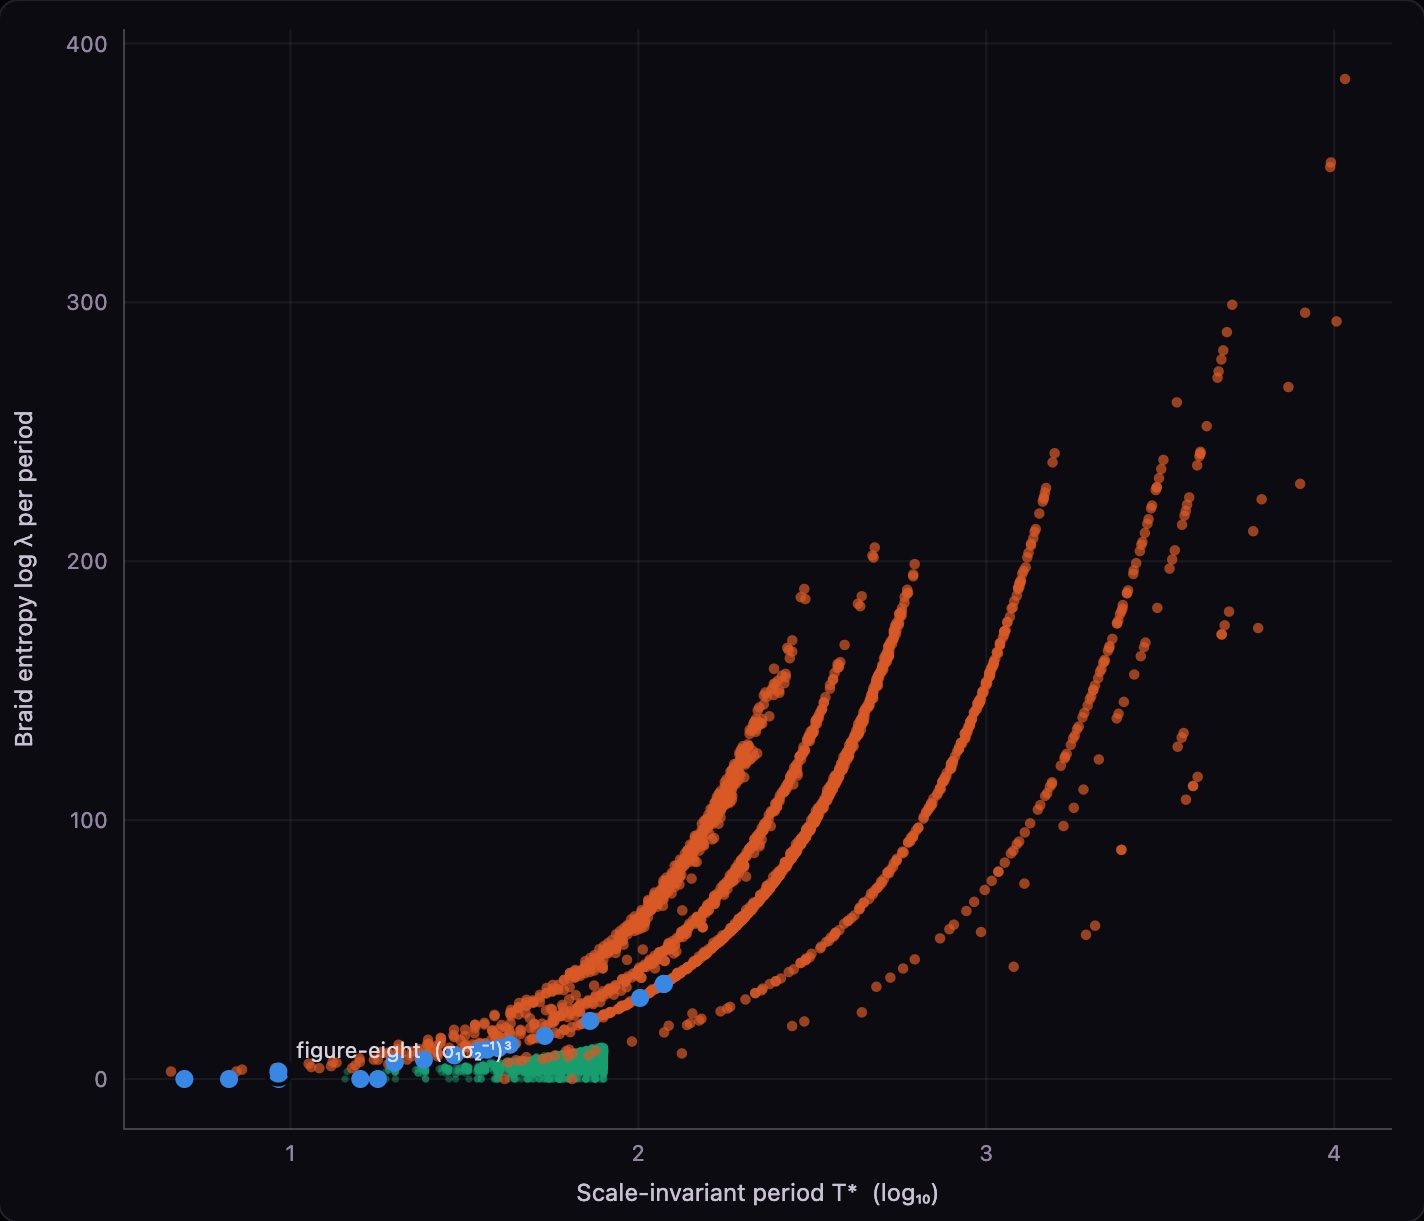
\includegraphics[width=0.49\linewidth]{docs/lab-entropy.jpg}\hfill
  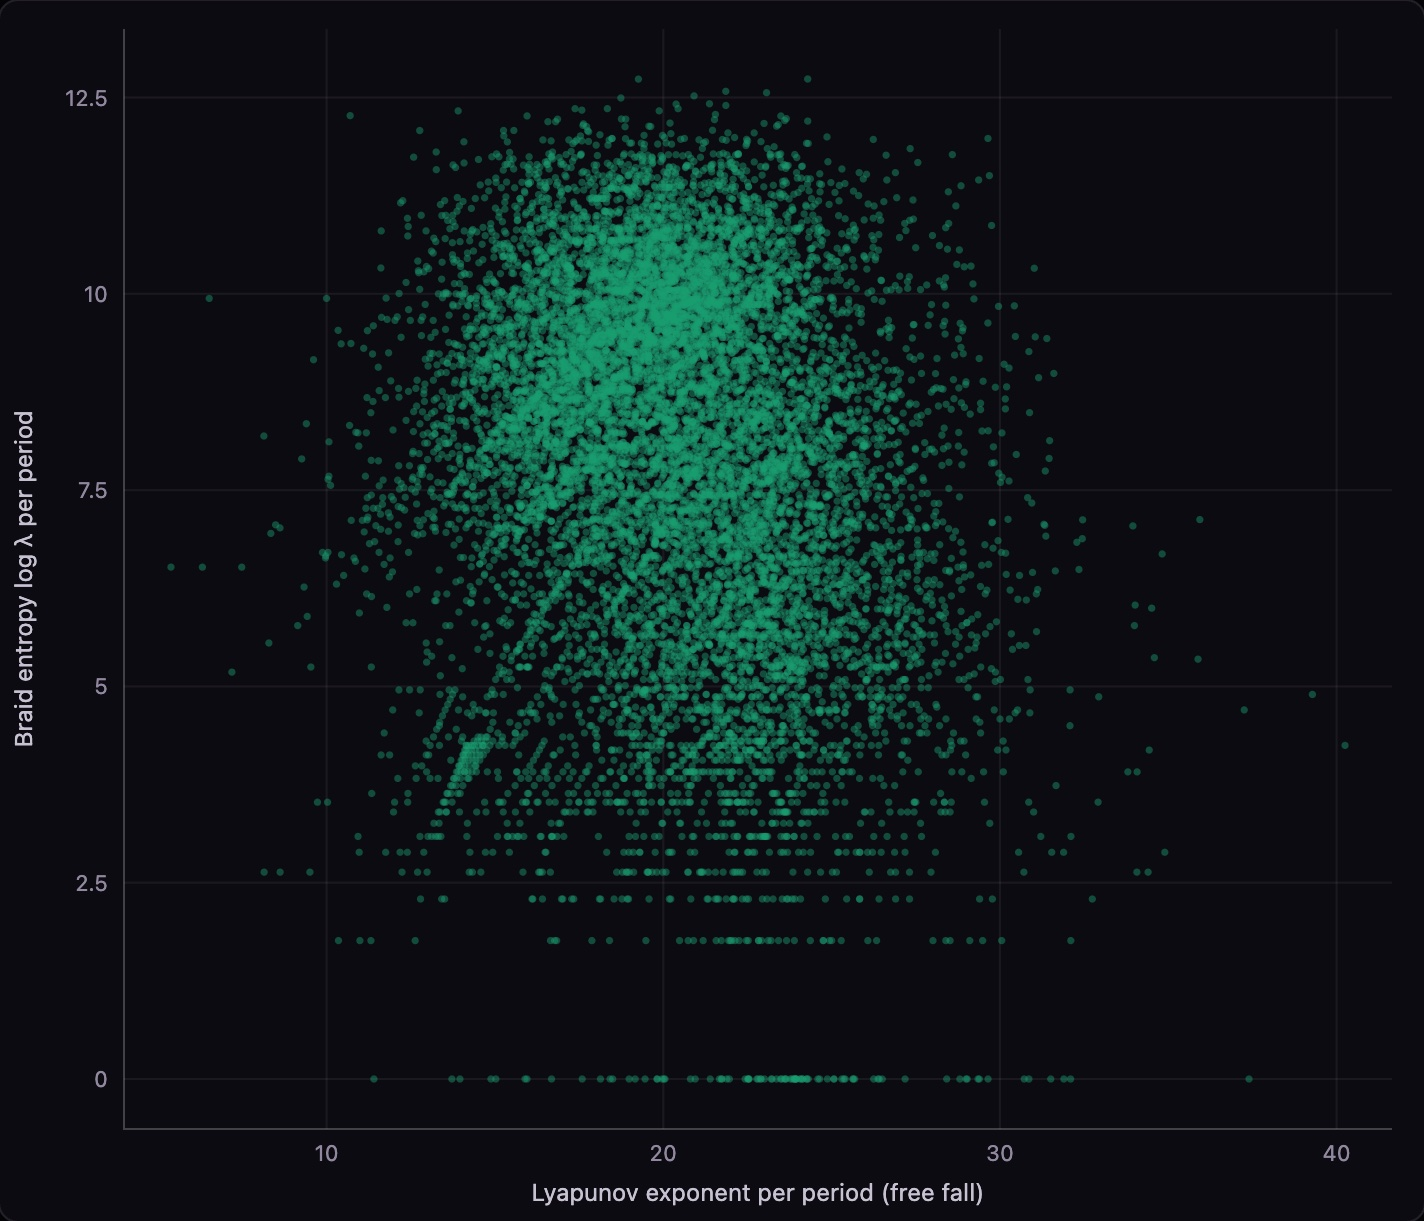
\includegraphics[width=0.49\linewidth]{docs/lab-lyapunov.jpg}
  \caption{The census in the instrument's Braid lab. Blue: classic orbits; orange: Li--Liao; green: free-fall
  (half-period braid). Left: braid entropy $\log\lambda_\beta$ against $\log_{10}T^*$. The Li--Liao orbits
  lie on separate curves, one per mass ratio; each is a straight line $\log\lambda_\beta=\kappa(m_3)T^*$ on
  linear axes. Right: for free-fall orbits, braid entropy against the published Lyapunov exponent per period;
  there is no correlation.}
  \label{fig:census}
\end{figure}

%=====================================================================
\section{Order of composition}
\label{sec:order}
%=====================================================================

A braid word is a time-ordered product, and reordering it generally changes the element. The same structure
governs how equations of motion are integrated, and the parallel is exact rather than metaphorical.

\subsection{Splitting and the Baker--Campbell--Hausdorff formula}

Write $H=T(\mathbf p)+V(\mathbf q)$ and let $A,B$ be the Liouville operators of $T$ and $V$. Their flows
(\emph{drift} and \emph{kick}) are exactly solvable but do not commute:
\begin{equation}
  e^{hA}e^{hB}=\exp\!\Bigl(h(A+B)+\tfrac{h^2}{2}[A,B]+\tfrac{h^3}{12}\bigl([A,[A,B]]-[B,[A,B]]\bigr)+\cdots\Bigr),
\end{equation}
where commutators of Liouville operators correspond to Poisson brackets such as $\{T,V\}$. Consequences:
\begin{itemize}[leftmargin=*]
\item kick-then-drift (symplectic Euler) is first order;
\item the symmetric composition $e^{\frac h2A}e^{hB}e^{\frac h2A}$ cancels all even-order terms; it is second
      order, time-reversible, and its error expands in powers of $h^2$ only;
\item updating positions and momenta from the old values simultaneously (explicit Euler) is not symplectic,
      and energy drifts secularly.
\end{itemize}
A symplectic integrator exactly conserves (in the sense of backward error analysis, up to exponentially
small terms) a nearby \emph{shadow Hamiltonian}
$\tilde H=H+h^2\bigl(c_1\{T,\{T,V\}\}+c_2\{V,\{T,V\}\}\bigr)+O(h^4)$, whose rational coefficients $c_1,c_2$ are
fixed by the order of the composition \cite{HairerLubichWanner2006,Yoshida1990}; changing the order changes
which shadow Hamiltonian is conserved.

In our instrument the order is load-bearing twice: the Bulirsch--Stoer extrapolation is performed in $h^2$,
which is valid only for the symmetric scheme, and the free-fall mirror construction relies on exact time
reversibility.

\subsection{Time-ordered products and holonomy}

In quantum mechanics the propagator is a time-ordered exponential $U=\mathcal T\exp(-i\!\int H\,dt)$; reordering
factors changes the result. The braid \eqref{eq:word} is the analogous time-ordered product of crossing
events. The correspondence is exact for flat connections on configuration spaces of points: the holonomy
(path-ordered exponential) of the Knizhnik--Zamolodchikov connection depends only on the braid of the path
and yields representations of $B_n$ \cite{KasselTuraev2008}.

\subsection{When order does not matter: Yang--Baxter}

What is special about $B_3$ is not only $\sigma_1\sigma_2\neq\sigma_2\sigma_1$ but the precise rule
$\sigma_1\sigma_2\sigma_1=\sigma_2\sigma_1\sigma_2$, the Yang--Baxter equation. In integrable one-dimensional
scattering it expresses that three-particle scattering is independent of the order of two-body collisions;
it underlies exactly solvable lattice models and the exchange statistics of anyons. The Newtonian three-body
problem is the opposite case: it is not integrable, and the order of close encounters changes the subsequent
motion, with nearby orders diverging exponentially. The braid records order topologically; the dynamics
punishes changes of order metrically.

%=====================================================================
\section{Birth and death of forms}
\label{sec:forms}
%=====================================================================

\subsection{The braid layer is a discrete factor}

Let $X$ be phase space with flow $\varphi_t$, and define the finite-time braid map
\begin{equation}
  B_\tau:X\to B_3,\qquad x\mapsto\text{braid of the world-lines of }\varphi_t(x),\ t\in[0,\tau].
\end{equation}
Strands in the plane cannot pass through each other except at a binary collision, so $B_\tau$ is locally
constant and changes only across collision boundaries. The two layers therefore have different stability:

\begin{center}
\begin{tabular}{@{}lll@{}}
\toprule
& trajectory layer & braid (form) layer\\
\midrule
state & continuous, $x\in X$ & discrete, $\beta\in B_3$\\
under perturbation & $\|\delta x(t)\|\approx e^{\lambda t}\|\delta x_0\|$ & unchanged until a jump\\
change & gradual & event (passage through collision)\\
\bottomrule
\end{tabular}
\end{center}

\noindent A form is robust in the short run (an open set of initial conditions shares it) and fragile in the
long run (the set realising a given form for $n$ crossings shrinks roughly like $e^{-hn}$). Its death is a
topological event, which is what makes it an object rather than a blur.

\subsection{Lifetimes from shadowing}

A periodic orbit $p$ with per-period braid $\beta_p$ is the ideal form: eternal but of measure zero. A nearby
trajectory shadows it \cite{Bowen1975}, reproducing $\beta_p\beta_p\beta_p\cdots$, until its deviation reaches
the margin $\delta$ to the nearest collision boundary:
\begin{equation}
  \tau_{\text{life}}\approx\frac1{\lambda_p}\ln\frac{\delta}{\varepsilon}.
  \label{eq:lifetime}
\end{equation}
Lifetime grows only logarithmically with precision. With $\lambda_p\approx15$ per period, $\varepsilon=10^{-6}$
and $\delta\approx0.1$, \eqref{eq:lifetime} gives $\tau\approx0.8$ periods, consistent with numerical
observation (iv) of Section~\ref{sec:instrument}.

\subsection{Which forms occur, and how often}

The number of braid words of length $n$ grows exponentially at the growth rate of $B_3$, whereas the number
realised by the dynamics grows like $e^{h_{\mathrm{top}}n}$ with a smaller entropy; the gap quantifies that most
forms never occur. Periodic-orbit theory weights each unstable orbit by the inverse of its stability multiplier
\cite{ChaosBook}, suggesting the frequency of a form
\begin{equation}
  P(\beta)\;\propto\sum_{p:\,\beta_p=\beta}e^{-\lambda_pT_p}.
\end{equation}
Since generic three-body systems eventually disintegrate, these are visits to a chaotic saddle; the lifetime of
the largest aggregate, the triple itself, is the ejection time first studied statistically by Agekyan and
Anosova \cite{AgekyanAnosova1968}.

\subsection{Aggregates as reducible braids}

The Nielsen--Thurston classification \cite{Thurston1988} gives the notion of an aggregate a precise meaning.
A braid is periodic, reducible or pseudo-Anosov. A \emph{reducible} braid preserves a curve enclosing a
subset of strands; for three bodies this is a binary plus a third body, with braid of the form
$\sigma_i^{2k}$ times an outer motion. The binary is an aggregate in the strict sense: a sub-braid that behaves
as a single strand at the coarser level. A pseudo-Anosov braid is an irreducibly entangled, democratic triple.
In a sliding window a trajectory's history becomes a sequence of phases, democratic, hierarchical and
near-periodic, and each transition is a discrete change of type. Braid-based detection of coherent clusters of
fluid trajectories uses the same idea \cite{Thiffeault2010,AllshouseThiffeault2012}. The census bears this
out. The only reducible closed orbits among the classics are the four hierarchical Broucke orbits
(Table~\ref{tab:types}).

\begin{remark}
The form layer depends on the window $\tau$: too short and nothing crosses, too long and every form has died.
Emergent objects live at an intermediate scale between the crossing time and $1/\lambda$, much like a
renormalisation scale. The time-zoom of the instrument moves through that scale.
\end{remark}

%=====================================================================
\section{Genealogical space}
\label{sec:genealogy}
%=====================================================================

\subsection{Cylinders of the free-fall problem}

Following Tanikawa and Mikkola \cite{TanikawaMikkola2015}, record at each syzygy (collinear configuration) the
label of the body in the middle. This defines a coding $\pi:D\to\Omega\subseteq\{1,2,3\}^{\N}$ from initial
conditions to symbol sequences. For a word $v$ of length $n$, the \emph{$n$-cylinder} $[v]$ is the set of
initial conditions whose history begins with $v$; its boundaries are binary collision curves, and the 3- and
4-cylinders are drawn in Fig.~10 of \cite{Hristov2024}. We equip $\Omega$ with
\begin{equation}
  \mu=\pi_\#\bigl(\text{normalised area on }D\bigr),
\end{equation}
which is the prior implicit in Agekyan and Anosova's statistical sampling.

Two features distinguish this tree from a generic one. It is a subshift: some words never occur (all
3-cylinders reported begin with~1). And histories may terminate (triple collision, measure zero) or freeze into
an eventually periodic tail when a binary escapes from the third body.

\subsection{The probability structure}

Let $H_n$ be the words of length $n$ and $\F_n=\sigma(\{[v]:v\in H_n\})$. For $\mu([v])>0$ define
$P_v=\mu(\,\cdot\mid[v])$ on $([v],\B([v]))$. The following hold.

\begin{proposition}[Genealogical consistency]\label{prop:consistency}
\begin{enumerate}[label=(\roman*)]
\item $\F_0\subseteq\F_1\subseteq\cdots$, and $\B(\Omega)=\sigma\bigl(\bigcup_n\F_n\bigr)$.
\item If $v$ has children $v_1,\dots,v_k$ and $q_i=\mu([v_i])/\mu([v])$, then $P_v=\sum_iq_iP_{v_i}$.
\item If $v\preceq w$ then $P_w=P_v(\,\cdot\mid[w])$.
\item Conversely, branching probabilities $q(e)$ summing to one at every node define
      $\mu([v])=\prod_{e\in\mathrm{path}(o,v)}q(e)$, which extends uniquely to a Borel probability measure
      (Kolmogorov extension).
\item For integrable $f$, $M_n=\E_\mu[f\mid\F_n]$ is a martingale, $M_n(\omega)=\int f\,dP_{v}$ for
      $\omega\in[v]$, $v\in H_n$, and $M_n\to f$ almost surely and in $L^1$ (L\'evy) \cite{Williams1991}.
\end{enumerate}
\end{proposition}

\noindent Let $h(v)=-\log\mu([v])$ be the surprisal of a node. For $a\preceq v$, $dP_v/dP_a=\mu([a])/\mu([v])$
on $[v]$, so
\begin{equation}
  \KL(P_v\,\|\,P_a)=h(v)-h(a).
\end{equation}
If $\pi_n$ truncates histories to depth $n$ and $D_n=\KL\bigl((\pi_n)_\#P_v\,\|\,(\pi_n)_\#P_a\bigr)$, then by
data processing $D_n\le D_{n+1}$, and in fact $D_n=h(v_n)-h(a)$ for $|a|\le n\le|v|$, where $v_n$ is the
depth-$n$ ancestor of $v$. More generally the chain rule
\begin{equation}
  \KL(P\,\|\,Q)=\KL\bigl(P^{(n)}\,\|\,Q^{(n)}\bigr)+\sum_{w\in H_n}P([w])\,\KL(P_w\,\|\,Q_w)
\end{equation}
splits divergence into the part visible at resolution $n$ and the part still hidden inside its classes.

\subsection{Two cautions specific to dynamics}

\paragraph{Convergence in $\Omega$ is not convergence in phase space.} Cylinders shrink to single histories in
$\Omega$, so $M_n\to f$ for observables that depend only on the symbolic history. For physical observables on
$D$ the limit is $\E[f\mid\F_\infty]$ with $\F_\infty=\pi^{-1}\B(\Omega)$, which equals $\B(D)$ only if the
syzygy partition is \emph{generating} (if $\pi$ is essentially injective). Escaping orbits, which share an
eventually periodic tail, suggest it is not. Whether the genealogy determines the physics is therefore a
dynamical question, the generating-partition problem of Kolmogorov--Sinai theory.

\paragraph{The coding is discontinuous on the binary collision curves.} In $\Omega$, histories are close when
they share a long prefix (ultrametric $d(\omega,\eta)=e^{-|\omega\wedge\eta|}$). Two physically close
initial conditions on opposite sides of a collision curve are immediately far apart genealogically.

\subsection{What the dynamics adds}

\paragraph{Surprisal grows at the entropy rate.} By the Shannon--\allowbreak McMillan--\allowbreak Breiman
theorem,
$h(v_n)/n\to h_\mu$ for $\mu$-almost every history, so $D_n$ grows linearly, with a slope set by the
dynamics. For an open (escaping) system the Kantz--Grassberger relation \cite{KantzGrassberger1985}
\begin{equation}
  \kappa=\sum\lambda^+-h_{\mathrm{KS}}
\end{equation}
ties the escape rate $\kappa$, the expansion rate and the entropy: probability mass lost from the tree equals
stretching that does not produce new branches.

\paragraph{Forms are infinite paths; lifetimes are meet depths.} Each of the 24{,}582 periodic i.c.s is a
point at the end of a nested chain $[p_1]\supset[p_2]\supset\cdots$. For a random history $\omega$, the depth
$|\omega\wedge p|$ is how long it imitates the form, so
\begin{equation}
  \Pr(\text{lifetime}\ge n)=\mu([p_n])=e^{-h(p_n)},
\end{equation}
linking the genealogical measure to the catalogued stability data.

\paragraph{Observation does not commute with conditioning.} Let $O$ map a history to ``which periodic
solution''. It is two-to-one: 24{,}582 i.c.s, 12{,}409 solutions. Each orbit has two genealogical addresses,
its dual i.c.s, which produce the same observed form; the 236 self-dual orbits are those whose two addresses
coincide. Hence $O_\#P_v\neq\nu(\,\cdot\mid O([v]))$ in general, and the dual pairs are a concrete instance.

%=====================================================================
\section{Time as refinement}
\label{sec:time}
%=====================================================================

\subsection{The tree is grown, not given}

The previous section treated $\Omega$ as given, a block universe in disguise. Dynamically, the tree is produced
by time. Let $\mathcal P$ be the partition of phase space by the first syzygy symbol and $\varphi$ the
one-symbol return map. The distinctions visible after $n$ steps form the join
\begin{equation}
  \mathcal P_n=\mathcal P\vee\varphi^{-1}\mathcal P\vee\cdots\vee\varphi^{-(n-1)}\mathcal P,
\end{equation}
whose cells are the $n$-cylinders. Each application of the dynamics splits every existing cell. The rate is
the Kolmogorov--Sinai entropy
\begin{equation}
  h_{\mathrm{KS}}=\lim_{n\to\infty}\frac1n H(\mathcal P_n),
\end{equation}
equal by Pesin's formula \cite{Pesin1977} to the sum of positive Lyapunov exponents: stretching carries ever
finer scales of the initial condition up to the observable scale. An initial condition known to precision
$\varepsilon$ fixes the history to depth $n\approx\log(1/\varepsilon)/h$; beyond $t\approx\log(1/\varepsilon)/\lambda$
later symbols are specified only as the dynamics produces them.

\subsection{K-systems and an internal time operator}

A flow is a Kolmogorov system if there is a $\sigma$-algebra $\F_0$ with
(i) $\F_0\subset\varphi\F_0\subset\varphi^2\F_0\subset\cdots$,
(ii) $\bigvee_n\varphi^n\F_0$ the full $\sigma$-algebra, and
(iii) $\bigwedge_n\varphi^{-n}\F_0$ trivial.
Misra, Prigogine and Courbage \cite{MisraPrigogineCourbage1979} showed that such systems admit an internal
time operator on observables,
\begin{equation}
  \mathsf T=\sum_n n\,(E_n-E_{n-1}),\qquad E_n=\E[\,\cdot\mid\varphi^n\F_0],\qquad
  U_t\,\mathsf T\,U_t^{-1}=\mathsf T+t ,
\end{equation}
where $U_t$ is the Koopman operator. Each eigenvalue labels the information that first appears at that level
of the tree. Time is then an operator whose spectrum indexes the growth of the genealogy, not merely a
coordinate on a static history.

\subsection{Becoming versus the block universe}

For Newtonian mechanics with real-number initial data the two pictures are empirically equivalent: Liouville's
theorem keeps fine-grained information constant, and what grows is distinguishability at fixed resolution. A
block-universe reading treats the filtration as \emph{revelation} of a history $\omega$ that exists in full.
For the tree to grow in fact, one more premise is needed:
\begin{itemize}[leftmargin=*]
\item \emph{finite information}: a physical state carries finitely many bits, so the deep cylinders are not
      decided at $t=0$ and become determined as the dynamics requires them; under this premise chaotic
      classical mechanics is effectively indeterministic \cite{DelSantoGisin2019}; or
\item a quantum description, where decoherent histories are cylinder-like sequences of coarse-grained
      projections and branching is part of the formalism \cite{GellMannHartle1990}.
\end{itemize}
The three-body problem makes the distinction vivid: at $\lambda\approx15$--$31$ per period, roughly fifty
digits of initial data are consumed within a few periods. Where those digits come from is where the two
pictures part.

\paragraph{Time-symmetric histories.} Free-fall orbits retrace themselves, and by
Proposition~\ref{prop:freefall} their full-period braid is trivial: they undo their own growth. A
growing-tree ontology accommodates them because they have measure zero; generic histories keep branching. The
arrow is not in the reversible equations but in the measure and the choice of a present $\F_0$ that time only
refines, the same structure as Boltzmann's account of the second law.

%=====================================================================
\section{Objects at finite resolution}
\label{sec:objects}
%=====================================================================

\subsection{Poincar\'e: displacement as compensable change}

Poincar\'e observed that two changes of impression, $A\to B$ and $A'\to B'$, may have nothing in common and yet
both count as ``the same displacement'', because the same correlative movement of the observer restores both
\cite{Poincare1902}. Let $S$ be the space of impressions and $M$ the observer's movements acting on $S$.

\begin{definition}
A change $a$ is a \emph{displacement} if there is $m\in M$ with $m\circ a=\mathrm{id}$ on impressions; two
changes are the same displacement if the same $m$ compensates both. Compensable changes form a group $G$, the
group of displacements. A \emph{solid object} is a structure whose changes lie in $G$; a \emph{deformation} is
a change no element of $G$ corrects.
\end{definition}

\noindent Poincar\'e adds that in a deformation each element undergoes a correctable change of position, but
the aggregate does not.

\subsection{Compensation has a tolerance}

Every observation has a resolution $\varepsilon$. With $O_\varepsilon$ the observation at resolution
$\varepsilon$, call $a$ an \emph{$\varepsilon$-displacement} if
\begin{equation}
  d\bigl(O_\varepsilon(m\circ a\circ x),\,O_\varepsilon(x)\bigr)\le\varepsilon\quad\text{for some }m\in M.
\end{equation}
The set $G_\varepsilon$ grows as $\varepsilon$ coarsens: a deforming blob, blurred enough, moves rigidly and is
``one thing''. $G_\varepsilon$ is only an approximate group, becoming exact in Poincar\'e's idealised limit.

\begin{definition}
Two parts belong to \emph{one object at scale $(\varepsilon,\tau)$} if their relative configuration stays within
$\varepsilon$ over the window $\tau$.
\end{definition}

\noindent Decreasing $\varepsilon$ or increasing $\tau$ can only split such objects, never merge them, so the
objects form an ultrametric hierarchy, the same kind of structure as the genealogical tree of
Section~\ref{sec:genealogy}. Parts identified only at coarse scale share only a shallow ancestor.

\subsection{Chaos makes scale and time dual}

Two parts at separation $\delta_0$ separate as $\delta_0e^{\lambda t}$, so they remain one object at resolution
$\varepsilon$ until
\begin{equation}
  t_{\text{split}}(\varepsilon)\approx\frac1\lambda\ln\frac{\varepsilon}{\delta_0}.
  \label{eq:split}
\end{equation}
The depth of their common ancestry is the logarithm of the resolution at which they are still one thing:
looking further into the future is equivalent to looking at finer scale. Two established quantities make this
precise. The finite-size Lyapunov exponent $\lambda(\delta)$ \cite{Aurell1997} is the separation rate measured at
scale $\delta$; it equals $\lambda_{\max}$ at fine scales and tends to zero at coarse scales, where separation
saturates and things look rigid. The $(\varepsilon,\tau)$-entropy per unit time $h(\varepsilon,\tau)$
\cite{GaspardWang1993} is the rate at which distinguishable histories appear at resolution $\varepsilon$, so
the number of objects distinguishable at scale $\varepsilon$ grows like
\begin{equation}
  N(\varepsilon,t)\sim e^{h(\varepsilon)\,t}.
\end{equation}
As time grows, we see more of the world.

\subsection{KAM tori are the solid objects of dynamics}

On an invariant KAM torus \cite{Kolmogorov1954,Arnold1963,Moser1962} the motion is conjugate to a translation
$\theta\mapsto\theta+\omega t$, a pure displacement in Poincar\'e's sense, compensable by the corresponding
rotation and with vanishing Lyapunov exponents. KAM tori move without splitting at any scale and persist under
perturbation. Chaotic layers are deformation: stretching and folding that no isometry corrects, measured by
positive exponents. The Oseledets splitting decomposes the tangent dynamics into neutral directions, where
compensation succeeds, and expanding and contracting directions, where it fails. A mixed phase space is
therefore a landscape of permanent objects embedded among forms that are born and die, and the resolution of
observation decides how much of the chaotic sea appears solid. This is also the honest limit of the
gravitational example: three-body phase space is mostly chaotic sea, so its forms are short-lived.

\subsection{Information and computation}

Splitting a class has a ledger. Information is produced at rate $h(\varepsilon,\tau)$; erasing a distinction
costs at least $k_BT\ln2$ per bit (Landauer \cite{Landauer1961}), while logically reversible computation avoids
that cost (Bennett \cite{Bennett1973}). Coarse-graining, merging objects, is the information-theoretic
counterpart of erasure; a reversible flow never truly merges, only the observer's resolution does. The object
hierarchy is thus something an observer maintains under a resource budget, and the appropriate successor of
classical mechanics for these questions is a mechanics of computation on information space.

%=====================================================================
\section{A computational programme}
\label{sec:programme}
%=====================================================================

Each step uses the integrator already validated in Section~\ref{sec:instrument}.

\begin{enumerate}[leftmargin=*]
\item \textbf{Braid words} (\emph{done}, Section~\ref{sec:census}). The braid $\beta$ and the invariants of
      Table~\ref{tab:invariants} for every catalogued orbit, validated against the published words and
      sequences.
\item \textbf{Topological Kepler law} (\emph{done}, Section~\ref{sec:census}). $\log\lambda_\beta$ is
      linear in $T^*$ within each mass ratio. Open: derive $\kappa(m_3)$, and find a closure-independent
      invariant for free-fall orbits.
\item \textbf{Cylinder tree.} Sample $\sim10^6$ uniform i.c.s in $D$, record their first $\sim12$ syzygy
      symbols, and estimate $q(w\mid v)$, $\mu([v])$ and the entropy rate $h(v_n)/n$.
\item \textbf{Markov test.} Cluster the continuation laws $\mathcal R_v\mu$ by KL divergence; finitely many
      clusters would indicate an effective Markov structure.
\item \textbf{Lifetimes.} Measure the meet depth $|\omega\wedge p|$ for ensembles near periodic orbits and test
      \eqref{eq:lifetime}: lifetime against $\ln(1/\varepsilon)$ should be linear with slope $1/\lambda_p$.
\item \textbf{Objects at scale.} Evolve clouds of $10^2$--$10^3$ nearby i.c.s, cluster them by
      $\varepsilon$-closeness over time, and measure $N(\varepsilon,t)$, the object dendrogram,
      $\lambda(\delta)$ and $h(\varepsilon)$, both near three-body periodic orbits and in the Chirikov standard
      map \cite{Chirikov1979}, where clouds on KAM tori should never split while clouds in the chaotic sea
      split at rate $h(\varepsilon)$, as predicted by \eqref{eq:split}.
\end{enumerate}

%=====================================================================
\section{Conclusion}
%=====================================================================

Starting from pictures of three-body orbits, we followed a single structure through several guises. Braids
turn trajectories into algebraic words whose invariants subsume the known topological classifications. Words
are time-ordered products, and order matters in the same mathematical sense in which it matters for
integrating Hamilton's equations. Chaos gives each braid a finite lifetime, so forms are born and die as
discrete events above a continuous substrate. The symbolic cylinders that index these forms carry a consistent
genealogical probability structure, and dynamics grows that genealogy at the rate of the Kolmogorov--Sinai
entropy, making time an operator of refinement rather than a coordinate on a completed history. Finally,
Poincar\'e's criterion of compensable change, relaxed to finite resolution, makes the very notion of a solid
object scale-dependent, and chaos couples scale to time: what is one thing now becomes many later. The
first of these statements, about braids, are now measurements. A census of 14{,}473 orbits, validated against the
published topology, shows the figure-eight to be the golden braid cubed. It finds a linear law between
topological entropy and period. It shows that the complexity of a form is independent of its instability.
The remaining proposals of Section~\ref{sec:programme} are designed to do the same for the genealogical and
scale-dependent claims.

%=====================================================================
\begin{thebibliography}{99}
%=====================================================================

\bibitem{AgekyanAnosova1968} T.~A. Agekyan and Zh.~P. Anosova, A study of the dynamics of triple systems by
means of statistical sampling, \emph{Soviet Astronomy} \textbf{11}, 1006 (1968).

\bibitem{AllshouseThiffeault2012} M.~R. Allshouse and J.-L. Thiffeault, Detecting coherent structures using
braids, \emph{Physica D} \textbf{241}, 95--105 (2012).

\bibitem{Arnold1963} V.~I. Arnold, Proof of a theorem of A.~N. Kolmogorov on the preservation of
conditionally periodic motions under a small perturbation of the Hamiltonian, \emph{Russian Math.\ Surveys}
\textbf{18}(5), 9--36 (1963).

\bibitem{Aurell1997} E.~Aurell, G.~Boffetta, A.~Crisanti, G.~Paladin and A.~Vulpiani, Predictability in the
large: an extension of the concept of Lyapunov exponent, \emph{J.\ Phys.\ A} \textbf{30}, 1--26 (1997).

\bibitem{Bennett1973} C.~H. Bennett, Logical reversibility of computation, \emph{IBM J.\ Res.\ Dev.}
\textbf{17}, 525--532 (1973).

\bibitem{Birman1974} J.~S. Birman, \emph{Braids, Links, and Mapping Class Groups}, Annals of Mathematics
Studies 82, Princeton University Press (1974).

\bibitem{Bowen1975} R.~Bowen, \emph{Equilibrium States and the Ergodic Theory of Anosov Diffeomorphisms},
Lecture Notes in Mathematics 470, Springer (1975).

\bibitem{BoylandArefStremler2000} P.~L. Boyland, H.~Aref and M.~A. Stremler, Topological fluid mechanics of
stirring, \emph{J.\ Fluid Mech.} \textbf{403}, 277--304 (2000).

\bibitem{ChaosBook} P.~Cvitanovi\'c, R.~Artuso, R.~Mainieri, G.~Tanner and G.~Vattay, \emph{Chaos: Classical
and Quantum}, Niels Bohr Institute, \url{https://ChaosBook.org}.

\bibitem{ChencinerMontgomery2000} A.~Chenciner and R.~Montgomery, A remarkable periodic solution of the
three-body problem in the case of equal masses, \emph{Ann.\ of Math.} \textbf{152}, 881--901 (2000).

\bibitem{Chirikov1979} B.~V. Chirikov, A universal instability of many-dimensional oscillator systems,
\emph{Phys.\ Rep.} \textbf{52}, 263--379 (1979).

\bibitem{DAlessandro1999} D.~D'Alessandro, M.~Dahleh and I.~Mezi\'c, Control of mixing in fluid flow: a maximum
entropy approach, \emph{IEEE Trans.\ Automat.\ Control} \textbf{44}, 1852--1863 (1999).

\bibitem{DelSantoGisin2019} F.~Del Santo and N.~Gisin, Physics without determinism: alternative
interpretations of classical physics, \emph{Phys.\ Rev.\ A} \textbf{100}, 062107 (2019).

\bibitem{FinnThiffeault2011} M.~D. Finn and J.-L. Thiffeault, Topological optimization of rod-stirring
devices, \emph{SIAM Review} \textbf{53}, 723--743 (2011).

\bibitem{GaspardWang1993} P.~Gaspard and X.-J. Wang, Noise, chaos, and $(\varepsilon,\tau)$-entropy per unit
time, \emph{Phys.\ Rep.} \textbf{235}, 291--343 (1993).

\bibitem{GellMannHartle1990} M.~Gell-Mann and J.~B. Hartle, Quantum mechanics in the light of quantum
cosmology, in \emph{Complexity, Entropy and the Physics of Information}, ed.\ W.~H. Zurek, Addison-Wesley
(1990).

\bibitem{HairerLubichWanner2006} E.~Hairer, C.~Lubich and G.~Wanner, \emph{Geometric Numerical Integration},
2nd ed., Springer (2006).

\bibitem{Hristov2024} I.~Hristov, R.~Hristova, V.~Dmitra\v{s}inovi\'c and K.~Tanikawa, Three-body periodic
collisionless equal-mass free-fall orbits revisited, \emph{Celest.\ Mech.\ Dyn.\ Astron.} \textbf{136}, 7
(2024); arXiv:2308.16159.

\bibitem{KantzGrassberger1985} H.~Kantz and P.~Grassberger, Repellers, semi-attractors, and long-lived chaotic
transients, \emph{Physica D} \textbf{17}, 75--86 (1985).

\bibitem{KasselTuraev2008} C.~Kassel and V.~Turaev, \emph{Braid Groups}, Graduate Texts in Mathematics 247,
Springer (2008).

\bibitem{Kolmogorov1954} A.~N. Kolmogorov, On the conservation of conditionally periodic motions under small
perturbation of the Hamiltonian, \emph{Dokl.\ Akad.\ Nauk SSSR} \textbf{98}, 527--530 (1954).

\bibitem{Landauer1961} R.~Landauer, Irreversibility and heat generation in the computing process, \emph{IBM J.\
Res.\ Dev.} \textbf{5}, 183--191 (1961).

\bibitem{LiJingLiao2018} X.~Li, Y.~Jing and S.~Liao, Over a thousand new periodic orbits of a planar
three-body system with unequal masses, \emph{Publ.\ Astron.\ Soc.\ Japan} \textbf{70}, 64 (2018).

\bibitem{LiLiao2017} X.~Li and S.~Liao, More than six hundred new families of Newtonian periodic planar
collisionless three-body orbits, \emph{Sci.\ China Phys.\ Mech.\ Astron.} \textbf{60}, 129511 (2017).

\bibitem{MikkolaTanikawa1999a} S.~Mikkola and K.~Tanikawa, Explicit symplectic algorithms for time-transformed
Hamiltonians, \emph{Celest.\ Mech.\ Dyn.\ Astron.} \textbf{74}, 287--295 (1999).

\bibitem{MikkolaTanikawa1999b} S.~Mikkola and K.~Tanikawa, Algorithmic regularization of the few-body problem,
\emph{Mon.\ Not.\ R.\ Astron.\ Soc.} \textbf{310}, 745--749 (1999).

\bibitem{MisraPrigogineCourbage1979} B.~Misra, I.~Prigogine and M.~Courbage, From deterministic dynamics to
probabilistic descriptions, \emph{Physica A} \textbf{98}, 1--26 (1979).

\bibitem{Montgomery1998} R.~Montgomery, The $N$-body problem, the braid group, and action-minimizing periodic
solutions, \emph{Nonlinearity} \textbf{11}, 363--376 (1998).

\bibitem{Moore1993} C.~Moore, Braids in classical gravity, \emph{Phys.\ Rev.\ Lett.} \textbf{70}, 3675--3679
(1993).

\bibitem{Moser1962} J.~Moser, On invariant curves of area-preserving mappings of an annulus, \emph{Nachr.\
Akad.\ Wiss.\ G\"ottingen, Math.-Phys.\ Kl.\ II}, 1--20 (1962).

\bibitem{Pesin1977} Ya.~B. Pesin, Characteristic Lyapunov exponents and smooth ergodic theory, \emph{Russian
Math.\ Surveys} \textbf{32}(4), 55--114 (1977).

\bibitem{Poincare1902} H.~Poincar\'e, \emph{La Science et l'Hypoth\`ese}, Flammarion (1902); English
translation \emph{Science and Hypothesis}.

\bibitem{SuvakovDmitrasinovic2013} M.~\v{S}uvakov and V.~Dmitra\v{s}inovi\'c, Three classes of Newtonian
three-body planar periodic orbits, \emph{Phys.\ Rev.\ Lett.} \textbf{110}, 114301 (2013).

\bibitem{TanikawaMikkola2015} K.~Tanikawa and S.~Mikkola, Symbol sequences and orbits of the free-fall
three-body problem, \emph{Publ.\ Astron.\ Soc.\ Japan} \textbf{67}, 115 (2015).

\bibitem{Thiffeault2010} J.-L. Thiffeault, Braids of entangled particle trajectories, \emph{Chaos} \textbf{20},
017516 (2010).

\bibitem{Thurston1988} W.~P. Thurston, On the geometry and dynamics of diffeomorphisms of surfaces,
\emph{Bull.\ Amer.\ Math.\ Soc.} \textbf{19}, 417--431 (1988).

\bibitem{Williams1991} D.~Williams, \emph{Probability with Martingales}, Cambridge University Press (1991).

\bibitem{Yoshida1990} H.~Yoshida, Construction of higher order symplectic integrators, \emph{Phys.\ Lett.\ A}
\textbf{150}, 262--268 (1990).

\end{thebibliography}

\end{document}
